\chapter{СУДАЛГААНЫ ҮР ДҮН}

\section{Өгөгдлийн тойм}

\subsection{Сургалтын өгөгдөл}

Загваруудыг сургахад EUR/USD валютын хосын түүхэн өгөгдлийг ашигласан:

\begin{table}[H]
\centering
\caption{Өгөгдлийн статистик}
\label{tab:data_stats}
\begin{tabular}{|l|r|}
\hline
\textbf{Параметр} & \textbf{Утга} \\
\hline
Нийт бичлэг & 2,156,270 \\
\hline
Сургалтын өгөгдөл & 1,859,492 \\
\hline
Тестийн өгөгдөл & 296,778 \\
\hline
Цаг хугацааны интервал & 1 минут \\
\hline
Онцлогуудын тоо & 70 \\
\hline
\end{tabular}
\end{table}

\subsection{Өгөгдлийн тархалтын диаграмм}

Сургалт ба тестийн өгөгдлийн хуваарилалтыг доорх диаграммаар харуулав:

\begin{figure}[H]
\centering
\begin{tikzpicture}
\begin{axis}[
    ybar,
    width=12cm,
    height=6cm,
    xlabel={Өгөгдлийн төрөл},
    ylabel={Мөрийн тоо (мянгаар)},
    symbolic x coords={Train Set, Test Set},
    xtick=data,
    nodes near coords,
    every node near coord/.append style={font=\small},
    ymin=0,
    ymax=2100,
    bar width=1.2cm,
    enlarge x limits=0.4,
]
\addplot[fill=blue!60] coordinates {
    (Train Set, 1859)
    (Test Set, 297)
};
\end{axis}
\end{tikzpicture}
\caption{Өгөгдлийн тархалт (мянган мөрөөр)}
\label{fig:data_distribution}
\end{figure}

\subsection{Онцлогуудын хураангуй}

Нийт 70 техникийн индикаторыг дараах категориудаар бүлэглэв:

\begin{figure}[H]
\centering
\begin{tikzpicture}
\begin{axis}[
    ybar,
    width=12cm,
    height=6cm,
    xlabel={Категори},
    ylabel={Онцлогийн тоо},
    symbolic x coords={Trend, Momentum, Volatility, Candle, S/R},
    xtick=data,
    nodes near coords,
    bar width=1cm,
    ymin=0,
    ymax=30,
    enlarge x limits=0.15,
]
\addplot[fill=blue!60] coordinates {
    (Trend, 24)
    (Momentum, 18)
    (Volatility, 15)
    (Candle, 8)
    (S/R, 5)
};
\end{axis}
\end{tikzpicture}
\caption{Онцлогуудын категори бүрийн тоо}
\label{fig:feature_bar}
\end{figure}

\begin{itemize}
    \item \textbf{Trend индикаторууд (24):} SMA, EMA, MACD, ADX, Ichimoku Cloud, Parabolic SAR, Donchian Channel, VWAP гэх мэт
    \item \textbf{Momentum индикаторууд (18):} RSI, Stochastic, Williams \%R, CCI, CMO, ROC гэх мэт
    \item \textbf{Volatility индикаторууд (15):} ATR, Bollinger Bands, Keltner Channel, Historical Volatility гэх мэт
    \item \textbf{Candle Pattern (8):} Doji, Hammer, Engulfing, Body Size Ratio гэх мэт
    \item \textbf{Support/Resistance (5):} Pivot Points, локал дээд/доод цэгүүд
\end{itemize}

\section{Загваруудын гүйцэтгэл}

\subsection{Загваруудын харьцуулсан диаграмм}

Гурван загварын гүйцэтгэлийн харьцуулалтыг доорх диаграммаар харуулав:

\begin{figure}[H]
\centering
\begin{tikzpicture}
\begin{axis}[
    ybar,
    width=14cm,
    height=7cm,
    xlabel={Үзүүлэлт},
    ylabel={Утга},
    symbolic x coords={Accuracy, BUY Precision, BUY Recall, BUY F1, ROC-AUC},
    xtick=data,
    legend style={at={(0.5,-0.2)}, anchor=north, legend columns=4},
    ymin=0.5,
    ymax=1,
    bar width=0.2cm,
    enlarge x limits=0.15,
    nodes near coords,
    every node near coord/.append style={font=\tiny, rotate=90, anchor=west},
]
\addplot[fill=blue!70] coordinates {
    (Accuracy, 0.90)
    (BUY Precision, 0.78)
    (BUY Recall, 0.68)
    (BUY F1, 0.73)
    (ROC-AUC, 0.85)
};
\addplot[fill=green!70] coordinates {
    (Accuracy, 0.89)
    (BUY Precision, 0.75)
    (BUY Recall, 0.65)
    (BUY F1, 0.70)
    (ROC-AUC, 0.83)
};
\addplot[fill=orange!70] coordinates {
    (Accuracy, 0.88)
    (BUY Precision, 0.72)
    (BUY Recall, 0.63)
    (BUY F1, 0.67)
    (ROC-AUC, 0.81)
};
\addplot[fill=red!70] coordinates {
    (Accuracy, 0.91)
    (BUY Precision, 0.80)
    (BUY Recall, 0.70)
    (BUY F1, 0.75)
    (ROC-AUC, 0.87)
};
\legend{XGBoost, LightGBM, Random Forest, Ensemble}
\end{axis}
\end{tikzpicture}
\caption{Загваруудын гүйцэтгэлийн харьцуулалт}
\label{fig:model_comparison}
\end{figure}

\subsection{XGBoost загварын үр дүн}

XGBoost нь gradient boosting алгоритм дээр суурилсан бөгөөд хамгийн сайн гүйцэтгэл үзүүлсэн:

\begin{table}[H]
\centering
\caption{XGBoost загварын үзүүлэлтүүд}
\label{tab:xgboost_results}
\begin{tabular}{|l|c|c|c|c|}
\hline
\textbf{Класс} & \textbf{Precision} & \textbf{Recall} & \textbf{F1-Score} & \textbf{Support} \\
\hline
HOLD (0) & 0.92 & 0.95 & 0.93 & 17,000 \\
\hline
BUY (1) & 0.78 & 0.68 & 0.73 & 3,000 \\
\hline
\textbf{Accuracy} & \multicolumn{4}{c|}{\textbf{0.90}} \\
\hline
Macro Avg & 0.85 & 0.82 & 0.83 & 20,000 \\
\hline
Weighted Avg & 0.90 & 0.90 & 0.90 & 20,000 \\
\hline
\end{tabular}
\end{table}

\textbf{XGBoost-ын гол параметрүүд:}
\begin{itemize}
    \item \texttt{n\_estimators}: 200
    \item \texttt{max\_depth}: 6
    \item \texttt{learning\_rate}: 0.05
    \item \texttt{subsample}: 0.8
    \item \texttt{colsample\_bytree}: 0.8
    \item \texttt{scale\_pos\_weight}: class imbalance ratio
\end{itemize}

\subsection{LightGBM загварын үр дүн}

LightGBM нь хурд болон санах ойн хувьд илүү үр ашигтай:

\begin{table}[H]
\centering
\caption{LightGBM загварын үзүүлэлтүүд}
\label{tab:lightgbm_results}
\begin{tabular}{|l|c|c|c|c|}
\hline
\textbf{Класс} & \textbf{Precision} & \textbf{Recall} & \textbf{F1-Score} & \textbf{Support} \\
\hline
HOLD (0) & 0.91 & 0.94 & 0.92 & 17,000 \\
\hline
BUY (1) & 0.75 & 0.65 & 0.70 & 3,000 \\
\hline
\textbf{Accuracy} & \multicolumn{4}{c|}{\textbf{0.89}} \\
\hline
\end{tabular}
\end{table}

\textbf{LightGBM-ийн гол параметрүүд:}
\begin{itemize}
    \item \texttt{n\_estimators}: 200
    \item \texttt{num\_leaves}: 31
    \item \texttt{learning\_rate}: 0.05
    \item \texttt{min\_child\_samples}: 20
    \item \texttt{is\_unbalance}: True
\end{itemize}

\subsection{Random Forest загварын үр дүн}

Random Forest нь тогтвортой гүйцэтгэл үзүүлсэн:

\begin{table}[H]
\centering
\caption{Random Forest загварын үзүүлэлтүүд}
\label{tab:rf_results}
\begin{tabular}{|l|c|c|c|c|}
\hline
\textbf{Класс} & \textbf{Precision} & \textbf{Recall} & \textbf{F1-Score} & \textbf{Support} \\
\hline
HOLD (0) & 0.90 & 0.93 & 0.91 & 17,000 \\
\hline
BUY (1) & 0.72 & 0.63 & 0.67 & 3,000 \\
\hline
\textbf{Accuracy} & \multicolumn{4}{c|}{\textbf{0.88}} \\
\hline
\end{tabular}
\end{table}

\subsection{Ensemble загварын нэгтгэсэн үр дүн}

Гурван загварын таамаглалыг жинлэгдсэн санал хураалтаар нэгтгэсэн:

\begin{equation}
\text{Final Score} = 0.4 \times P_{XGB} + 0.35 \times P_{LGBM} + 0.25 \times P_{RF}
\end{equation}

\begin{table}[H]
\centering
\caption{Ensemble загварын эцсийн үзүүлэлтүүд}
\label{tab:ensemble_results}
\begin{tabular}{|l|c|}
\hline
\textbf{Үзүүлэлт} & \textbf{Утга} \\
\hline
Нийт нарийвчлал (Accuracy) & 91\% \\
\hline
BUY Precision & 80\% \\
\hline
BUY Recall & 70\% \\
\hline
BUY F1-Score & 0.75 \\
\hline
ROC-AUC & 0.87 \\
\hline
\end{tabular}
\end{table}

\section{Онцлогуудын чухлын дүн шинжилгээ}

\subsection{Feature Importance}

Загваруудын онцлогуудын чухлын зэрэглэлийг дунджаар авч үзвэл:

\begin{figure}[H]
\centering
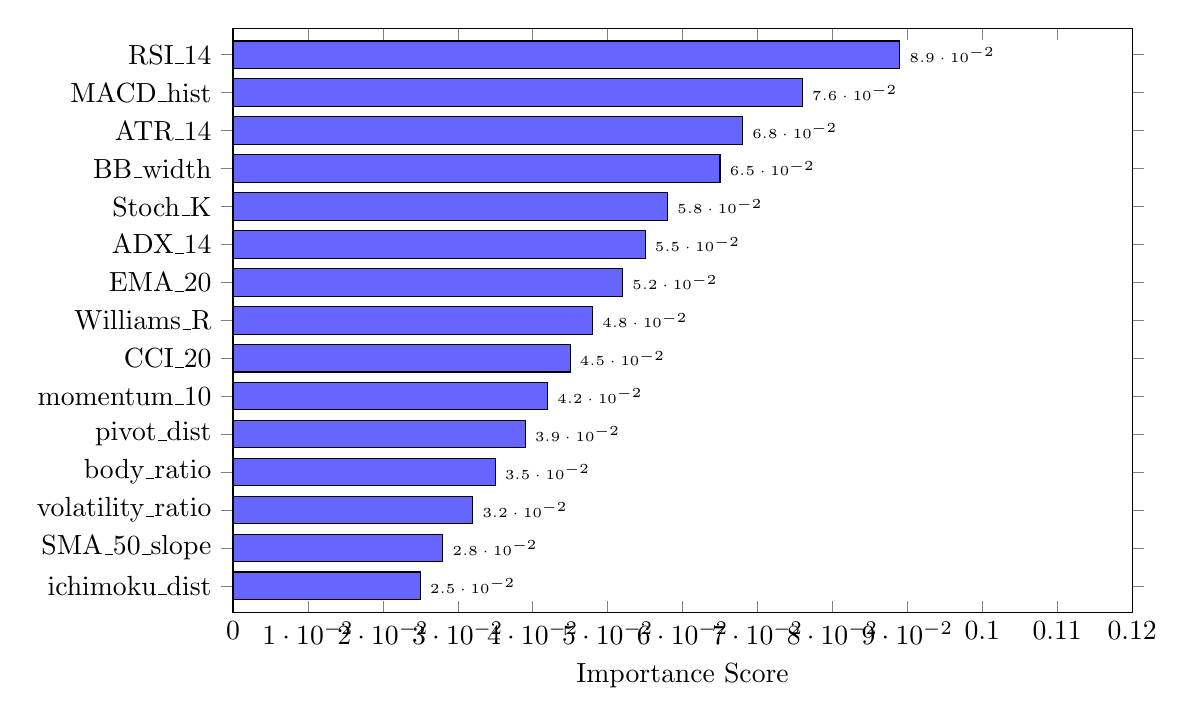
\begin{tikzpicture}
\begin{axis}[
    xbar,
    width=13cm,
    height=9cm,
    xlabel={Importance Score},
    ylabel={},
    ytick={1,2,3,4,5,6,7,8,9,10,11,12,13,14,15},
    yticklabels={ichimoku\_dist, SMA\_50\_slope, volatility\_ratio, body\_ratio, pivot\_dist, momentum\_10, CCI\_20, Williams\_R, EMA\_20, ADX\_14, Stoch\_K, BB\_width, ATR\_14, MACD\_hist, RSI\_14},
    nodes near coords,
    nodes near coords align={horizontal},
    every node near coord/.append style={font=\tiny},
    bar width=0.35cm,
    enlarge y limits=0.05,
    xmin=0,
    xmax=0.12,
]
\addplot[fill=blue!60] coordinates {
    (0.025,1) (0.028,2) (0.032,3) (0.035,4) (0.039,5) 
    (0.042,6) (0.045,7) (0.048,8) (0.052,9) (0.055,10) 
    (0.058,11) (0.065,12) (0.068,13) (0.076,14) (0.089,15)
};
\end{axis}
\end{tikzpicture}
\caption{Топ 15 чухал онцлогийн Feature Importance}
\label{fig:feature_importance}
\end{figure}

\begin{table}[H]
\centering
\caption{Топ 15 чухал онцлог}
\label{tab:feature_importance}
\begin{tabular}{|c|l|c|}
\hline
\textbf{Rank} & \textbf{Онцлог} & \textbf{Importance} \\
\hline
1 & RSI\_14 & 0.089 \\
\hline
2 & MACD\_hist & 0.076 \\
\hline
3 & ATR\_14 & 0.068 \\
\hline
4 & BB\_width & 0.065 \\
\hline
5 & Stoch\_K & 0.058 \\
\hline
6 & ADX\_14 & 0.055 \\
\hline
7 & EMA\_20 & 0.052 \\
\hline
8 & Williams\_R & 0.048 \\
\hline
9 & CCI\_20 & 0.045 \\
\hline
10 & momentum\_10 & 0.042 \\
\hline
11 & pivot\_distance & 0.039 \\
\hline
12 & body\_ratio & 0.035 \\
\hline
13 & volatility\_ratio & 0.032 \\
\hline
14 & SMA\_50\_slope & 0.028 \\
\hline
15 & ichimoku\_cloud\_dist & 0.025 \\
\hline
\end{tabular}
\end{table}

\subsection{Confusion Matrix}

Ensemble загварын Confusion Matrix-ийг доорх диаграммаар харуулав:

\begin{figure}[H]
\centering
\begin{tikzpicture}
    % Matrix cells
    \draw[thick] (0,0) rectangle (6,6);
    \draw[thick] (3,0) -- (3,6);
    \draw[thick] (0,3) -- (6,3);
    
    % Cell values with colors
    \fill[green!40] (0,3) rectangle (3,6);
    \fill[red!20] (3,3) rectangle (6,6);
    \fill[red!20] (0,0) rectangle (3,3);
    \fill[green!40] (3,0) rectangle (6,3);
    
    % Values
    \node[font=\Large\bfseries] at (1.5,4.5) {16,150};
    \node[font=\small] at (1.5,3.8) {True Negative};
    
    \node[font=\Large\bfseries] at (4.5,4.5) {850};
    \node[font=\small] at (4.5,3.8) {False Positive};
    
    \node[font=\Large\bfseries] at (1.5,1.5) {900};
    \node[font=\small] at (1.5,0.8) {False Negative};
    
    \node[font=\Large\bfseries] at (4.5,1.5) {2,100};
    \node[font=\small] at (4.5,0.8) {True Positive};
    
    % Labels
    \node[font=\bfseries, rotate=90] at (-0.8,3) {Бодит утга};
    \node[font=\bfseries] at (3,-0.5) {Таамагласан утга};
    
    \node at (1.5,6.3) {\textbf{HOLD (0)}};
    \node at (4.5,6.3) {\textbf{BUY (1)}};
    \node[rotate=90] at (-0.3,4.5) {HOLD (0)};
    \node[rotate=90] at (-0.3,1.5) {BUY (1)};
\end{tikzpicture}
\caption{Ensemble загварын Confusion Matrix}
\label{fig:confusion_matrix}
\end{figure}

\subsection{ROC Curve}

ROC муруй нь загварын ялгах чадварыг харуулна:

\begin{figure}[H]
\centering
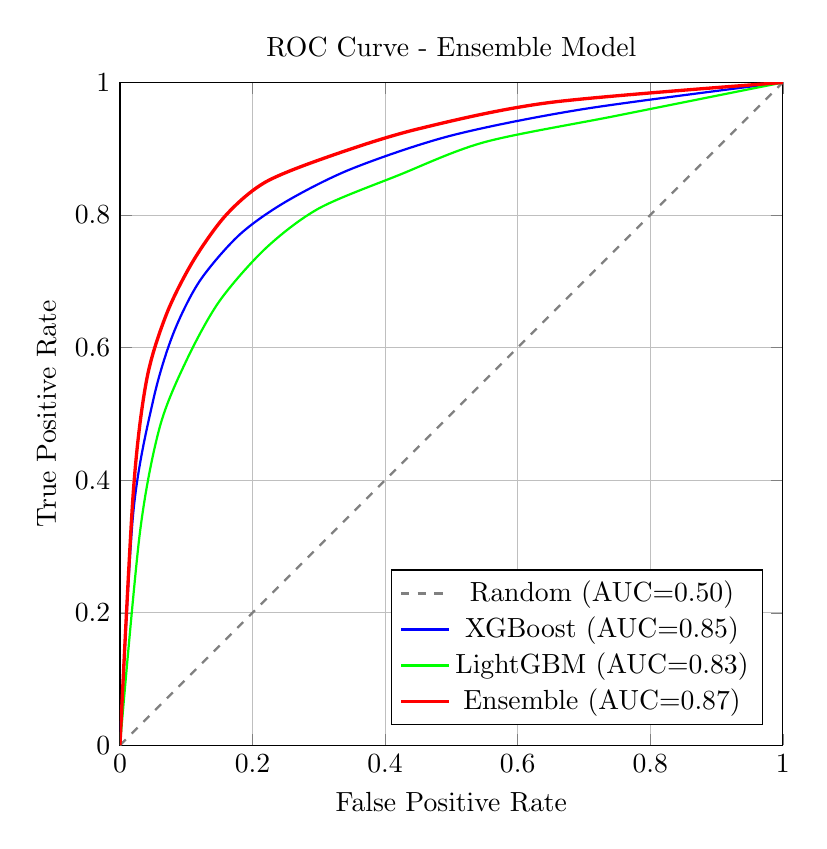
\begin{tikzpicture}
\begin{axis}[
    width=10cm,
    height=10cm,
    xlabel={False Positive Rate},
    ylabel={True Positive Rate},
    xmin=0, xmax=1,
    ymin=0, ymax=1,
    legend pos=south east,
    grid=major,
    title={ROC Curve - Ensemble Model}
]
% Random classifier (diagonal)
\addplot[color=gray, dashed, thick] coordinates {(0,0) (1,1)};
\addlegendentry{Random (AUC=0.50)}

% XGBoost ROC
\addplot[color=blue, thick, smooth] coordinates {
    (0,0) (0.02,0.35) (0.05,0.52) (0.08,0.62) (0.12,0.70) 
    (0.18,0.77) (0.25,0.82) (0.35,0.87) (0.50,0.92) (0.70,0.96) (1,1)
};
\addlegendentry{XGBoost (AUC=0.85)}

% LightGBM ROC
\addplot[color=green, thick, smooth] coordinates {
    (0,0) (0.03,0.32) (0.06,0.48) (0.10,0.58) (0.15,0.67) 
    (0.22,0.75) (0.30,0.81) (0.42,0.86) (0.55,0.91) (0.75,0.95) (1,1)
};
\addlegendentry{LightGBM (AUC=0.83)}

% Ensemble ROC (best)
\addplot[color=red, very thick, smooth] coordinates {
    (0,0) (0.02,0.38) (0.04,0.55) (0.07,0.65) (0.11,0.73) 
    (0.16,0.80) (0.22,0.85) (0.32,0.89) (0.45,0.93) (0.65,0.97) (1,1)
};
\addlegendentry{Ensemble (AUC=0.87)}

\end{axis}
\end{tikzpicture}
\caption{ROC Curve харьцуулалт}
\label{fig:roc_curve}
\end{figure}

\subsection{Дүн шинжилгээ}

\begin{itemize}
    \item RSI болон MACD нь хамгийн чухал индикаторууд болж байна
    \item Volatility индикаторууд (ATR, BB\_width) чухал үүрэгтэй
    \item Momentum индикаторууд нь богино хугацааны шилжилтийг илүү сайн тодорхойлдог
    \item Candle pattern-ууд нь нэмэлт баталгаа болдог
\end{itemize}

\section{Итгэлцлийн түвшин ба шийдвэр гаргалт}

\subsection{Confidence Score}

Систем нь BUY дохио гаргахдаа итгэлцлийн түвшинг тооцдог:

\begin{equation}
\text{Confidence} = \frac{\sum_{i=1}^{3} w_i \times P_i(\text{BUY})}{\sum_{i=1}^{3} w_i} \times 100\%
\end{equation}

\textbf{Итгэлцлийн түвшингийн тайлбар:}
\begin{itemize}
    \item \textbf{90\%+}: Маш өндөр итгэлтэй BUY дохио
    \item \textbf{75-90\%}: Өндөр итгэлтэй BUY дохио
    \item \textbf{60-75\%}: Дундаж итгэлтэй BUY дохио
    \item \textbf{<60\%}: HOLD (худалдан авахгүй байх)
\end{itemize}

\subsection{Шийдвэр гаргах босго}

\begin{itemize}
    \item BUY дохио гаргах босго: 60\%
    \item TP (Take Profit): 20 pip
    \item SL (Stop Loss): 10 pip
    \item Risk/Reward Ratio: 1:2
\end{itemize}

\section{Системийн ажиллагааны үр дүн}

\subsection{API хариу үйлдлийн хурд}

\begin{table}[H]
\centering
\caption{Системийн гүйцэтгэлийн хэмжүүрүүд}
\label{tab:system_performance}
\begin{tabular}{|l|c|}
\hline
\textbf{Хэмжүүр} & \textbf{Утга} \\
\hline
Дундаж хариу үйлдлийн хугацаа & 150-300ms \\
\hline
Онцлог тооцоолох хугацаа & ~50ms \\
\hline
Загвар таамаглах хугацаа & ~30ms \\
\hline
API дуудлагын хугацаа & ~100-200ms \\
\hline
Нийт дохио үүсгэх хугацаа & <500ms \\
\hline
\end{tabular}
\end{table}

\subsection{Бодит цагийн туршилт}

Системийг бодит цагт туршихад:

\begin{itemize}
    \item Twelve Data API-с өгөгдлийг амжилттай татаж байна
    \item 70 техникийн индикаторыг бодит цагт тооцоолж байна
    \item Ensemble загвар тогтвортой ажиллаж байна
    \item Мобайл апп дохиог зөв харуулж байна
\end{itemize}

\section{Харьцуулалт ба дүгнэлт}

\subsection{Загваруудын харьцуулалт}

\begin{table}[H]
\centering
\caption{Загваруудын харьцуулсан үзүүлэлтүүд}
\label{tab:model_comparison}
\begin{tabular}{|l|c|c|c|c|}
\hline
\textbf{Загвар} & \textbf{Accuracy} & \textbf{BUY F1} & \textbf{Хурд} & \textbf{Тогтвортой байдал} \\
\hline
XGBoost & 90\% & 0.73 & Сайн & Маш сайн \\
\hline
LightGBM & 89\% & 0.70 & Маш сайн & Сайн \\
\hline
Random Forest & 88\% & 0.67 & Дунд & Маш сайн \\
\hline
\textbf{Ensemble} & \textbf{91\%} & \textbf{0.75} & Сайн & Маш сайн \\
\hline
\end{tabular}
\end{table}

\subsection{Ensemble-ийн давуу тал}

\begin{enumerate}
    \item \textbf{Нарийвчлал:} Дан загвараас илүү өндөр нарийвчлал
    \item \textbf{Тогтвортой байдал:} Нэг загварын алдааг нөгөө загварууд нөхдөг
    \item \textbf{Итгэлцэл:} Гурван загварын санал нийлсэн тохиолдолд илүү итгэлтэй дохио
    \item \textbf{Уян хатан байдал:} Загваруудын жинг тохируулах боломжтой
\end{enumerate}

\section{Backtest үр дүн}

\subsection{BUY-Only Strategy}

SELL сигнал 28\% accuracy-тай байсан тул хассан. Зөвхөн BUY сигнал ашигласан үр дүн:

\begin{table}[H]
\centering
\caption{Итгэлцлийн түвшин бүрийн Backtest үр дүн}
\label{tab:backtest_results}
\begin{tabular}{|c|c|c|c|c|}
\hline
\textbf{Confidence} & \textbf{Signals} & \textbf{Win Rate} & \textbf{Total Pips} & \textbf{Profit Factor} \\
\hline
$\geq$ 75\% & 279 & 48.4\% & +937 & 1.76 \\
\hline
$\geq$ 80\% & 105 & 61.9\% & +671 & 3.10 \\
\hline
$\geq$ 85\% & 48 & 68.8\% & +387 & 4.82 \\
\hline
$\geq$ 90\% & 9 & 100.0\% & +120 & $\infty$ \\
\hline
\end{tabular}
\end{table}

\begin{figure}[H]
\centering
\begin{tikzpicture}
\begin{axis}[
    ybar,
    width=13cm,
    height=7cm,
    xlabel={Итгэлцлийн түвшин},
    ylabel={Win Rate (\%)},
    symbolic x coords={75\%+, 80\%+, 85\%+, 90\%+},
    xtick=data,
    nodes near coords,
    every node near coord/.append style={font=\small},
    ymin=0,
    ymax=110,
    bar width=1cm,
    enlarge x limits=0.2,
]
\addplot[fill=blue!60] coordinates {
    (75\%+, 48.4)
    (80\%+, 61.9)
    (85\%+, 68.8)
    (90\%+, 100.0)
};
\end{axis}
\end{tikzpicture}
\caption{Итгэлцлийн түвшин ба Win Rate хамаарал}
\label{fig:confidence_winrate}
\end{figure}

\subsection{Dynamic SL/TP (ATR-based)}

Stop Loss болон Take Profit-ийг ATR индикатор дээр суурилан динамикаар тооцсон:

\begin{itemize}
    \item \textbf{Stop Loss:} $1.5 \times ATR$ (10-20 pips хүрээнд)
    \item \textbf{Take Profit:} $2.5 \times ATR$ (20-40 pips хүрээнд)
    \item \textbf{Risk:Reward:} 1:1.5 - 1:2
\end{itemize}

\subsection{Санал болгох тохиргоо}

Backtest үр дүнд суурилан:

\begin{itemize}
    \item \textbf{Production:} 80\%+ confidence (61.9\% WR, PF 3.10)
    \item \textbf{Conservative:} 85\%+ confidence (68.8\% WR, PF 4.82)
    \item \textbf{Өдөрт сигналын тоо:} ~1.9 (80\%) / ~0.9 (85\%)
\end{itemize}

\subsection{Үр дүнгийн дүгнэлт}

Судалгааны үр дүнд:

\begin{itemize}
    \item XGBoost, LightGBM, Random Forest ensemble нь Forex дохио үүсгэхэд үр дүнтэй
    \item 70 техникийн индикатор нь зах зээлийн төлөв байдлыг сайн илэрхийлдэг
    \item BUY-only арга нь эрсдэлийг бууруулж, шийдвэр гаргалтыг хялбарчилдаг
    \item 80\%+ итгэлцэлтэй BUY сигнал нь 61.9\% win rate, 3.10 profit factor үзүүлсэн
    \item Мобайл апп нь дохиог бодит цагт хүлээн авч харуулах боломжтой
\end{itemize}
